\documentclass[12pt,a4paper]{article}
\usepackage[utf8]{inputenc}
\usepackage[T1]{fontenc}
\usepackage{comment}
\date{} 
\usepackage[spanish]{babel}
\usepackage{amsmath}
\usepackage{amsfonts}

\usepackage{tcolorbox} %cajas de definiciones
\usepackage{color}%resaltador
\usepackage{soul}%resaltador


%para crear sub sub sub titulos
\makeatletter
\renewcommand\paragraph{\@startsection{paragraph}{4}{\z@}%
            {-2.5ex\@plus -1ex \@minus -.25ex}%
            {1.25ex \@plus .25ex}%
            {\normalfont\normalsize\bfseries}}
\makeatother
\setcounter{secnumdepth}{4} % how many sectioning levels to assign numbers to
\setcounter{tocdepth}{4}    % how many sectioning levels to show in ToC

\usepackage[none]{hyphenat} %para que no corte las palabras al final del renglon
\usepackage{amssymb}
\usepackage{graphicx}
\usepackage{caption}
\usepackage{mwe}
\usepackage{url} %url
\usepackage{hyperref} %indice con hipervínculo
\hypersetup{
    colorlinks=true,
    linkcolor=black,
    filecolor=white,      
    urlcolor=blue,
}
\usepackage{float} 
\usepackage{mathpazo} % Palatino font
\usepackage[left=2.50cm, right=2.50cm, top=1.50cm, bottom=1.50cm]{geometry}
\author{Caamiña, Daniela \and Yapura, Cristian}
\title{Trabajo final \\Automatización industrial}
\graphicspath{ {images/} }
	
\begin{document}
\begin{titlepage} %Carátula 			
	\newcommand{\HRule}{\rule{\linewidth}{0.5mm}}
	\center % Centre everything on the page		
	\textsc{\LARGE Universidad Nacional de la Patagonia San Juan Bosco}\\[1.5cm]
	\textsc{\Large Automatización Industrial}\\[0.5cm]
	\textsc{\large Trabajo Final}\\[0.5cm]
	\HRule\\[0.4cm]
	\huge\bfseries{Banco de pruebas para motor trifásico}\\[0.2cm]
	\HRule\\[1.5cm]
	\begin{minipage}{0.4\textwidth}
		\begin{flushleft}
			\large
			\textit{Alumnos}\\
			\textsc{Caamiña,} Daniela \\
			\textsc{Yapura,} Cristian
		\end{flushleft}
	\end{minipage}
	\begin{minipage}{0.4\textwidth}
		\begin{flushright}
			\large
			\textit{Docentes}\\
			Ing. \textsc{Lorenc,} Marcelo \\
			Dr. \textsc{Peña,} Ramiro
		\end{flushright}
	\end{minipage}
	\vfill\vfill\vfill
	\large{MES AÑO}
	\vfill\vfill
	\includegraphics[width=0.2\textwidth]{unpsjb.png}\\[1cm]
	\vfill
\end{titlepage}

\tableofcontents
\newpage

\listoffigures
\newpage

\section*{Lista de Acrónimos}
\noindent
\textbf{CANOpen:} \textit{}\\
\textbf{HMI:} \textit{Interfaz Humano-máquina}\\
\textbf{MBE :} \textit{}\\
\textbf{Modbus:} \textit{Modicon Bus}\\
\textbf{PDO :} \textit{Objetos de Datos de Proceso}\\
\textbf{PLC :} \textit{Controlador Lógico Programable}\\
\textbf{SCADA :} \textit{Supervisión, Control y Adquisición de Datos}\\ %desactiva sangria solo para este parrafo
\textbf{SDO :} \textit{Objetos de Datos de Servicio}\\
\textbf{ :} \textit{}\\
\textbf{ :} \textit{}\\
\textbf{ :} \textit{}\\
\textbf{ :} \textit{}\\
\textbf{ :} \textit{}\\
\textbf{ :} \textit{}\\

\newpage
\sloppy %para justificar los párrafos

\section{Introducción}
En el Laboratorio de Fluidos de la Universidad, se utiliza el Túnel de Viento para realizar el contraste de anemómetros y experimentos para distintas materias. Gran parte de estas aplicaciones requieren que se conozca la velocidad del fluido (aire). Por lo tanto, variación de presión, humedad, presión atmosférica y temperatura son variables requeridas para lograr estimarla con mayor precisión.
Cada variable debe ser medida de forma manual con sus respectivos instrumentos para luego ingresar estos valores a una tabla (generada de forma estadística) y obtener una estimación de la velocidad del fluido.\\

El túnel en sus comienzos, para realizar distintas mediciones, utilizaba un control de velocidad a lazo abierto en el que se modificaba la resistencia del motor, para cambiar la velocidad del aire en pasos discretos. Actualmente, desde principios del año 2020 se utiliza un variador de velocidad de la marca \textbf{Long Shenq}, con él se obtiene un control mas continuo en la frecuencia del motor. \\

Realizar este proceso de forma manual, se torna engorroso y poco práctico para la realización de varias mediciones por lo que se realiza este trabajo final de carrera para realizar la \textit{Automatización del Túnel de Viento de la UNPSJB}.

\newpage

\section{Objetivo}
Un banco de pruebas de un motor cuenta con un punto de apoyo donde se conecta el motor y sus componentes mecánicos, ademas dentro de esta plataforma existe un sistema de medición que posee sensores, variador y PLC para los procedimientos de prueba.
Un banco de pruebas puede ser un prototipo de un gran desarrollo industrial o simplemente un banco formado para realizar pruebas educativas. \\

El objetivo de este trabajo final para la cátedra de Automatización Industrial es construir un banco de pruebas para ser utilizado por cualquier persona dentro el laboratorio de Automatización y Control. Se espera generar un banco de pruebas que cuente con:
\begin{itemize}
    \item Motor trifásico 1,5kW (Altium)\textit{-Proporcionado por la cátedra-}
    \item PLC (Schneider - M340) \textit{-Proporcionado por la cátedra-}
    \item Variador de velocidad (Schneider - ATV312 ) \textit{-Proporcionado por la cátedra-}
    \item Panel de control
        \subitem Botón de emergencia
        \subitem Encendido/ apagado
        \subitem Potenciómetro para variar velocidad
        \subitem Display para observar velocidad
        \subitem Alarmas visuales
    \item HMI
        \subitem Alarmas
        \subitem Información en tiempo real
        \subitem Histórico de datos
        \subitem Control general del banco
\end{itemize}

\newpage

\section{Elementos}
\subsection{Motor}
\subsubsection{Especificaciones}

	El motor (Figura \ref{fig:motor}) asincrónico que se utiliza es de la marca \textbf{Altium} perteneciente a la firma \textbf{Schneider Electric}. Las especificaciones se muestran a continuación \\
	\paragraph*{Altium Eff2}
	\begin{itemize}
		\item 	Tipo: TE2A90SP2
		\item   Tensión nominal: 220/380 V
		\item 	Corriente nominal: 5.97 A 
		\item	Frecuencia nominal:  50 Hz.
		\item 	Potencia: 1.5kW / 2 HP
		\item 	Fases: 3
		\item   Factor de Potencia: 0.84
	\end{itemize}
	\newpage
	\begin{figure}[h!]
		\centering
		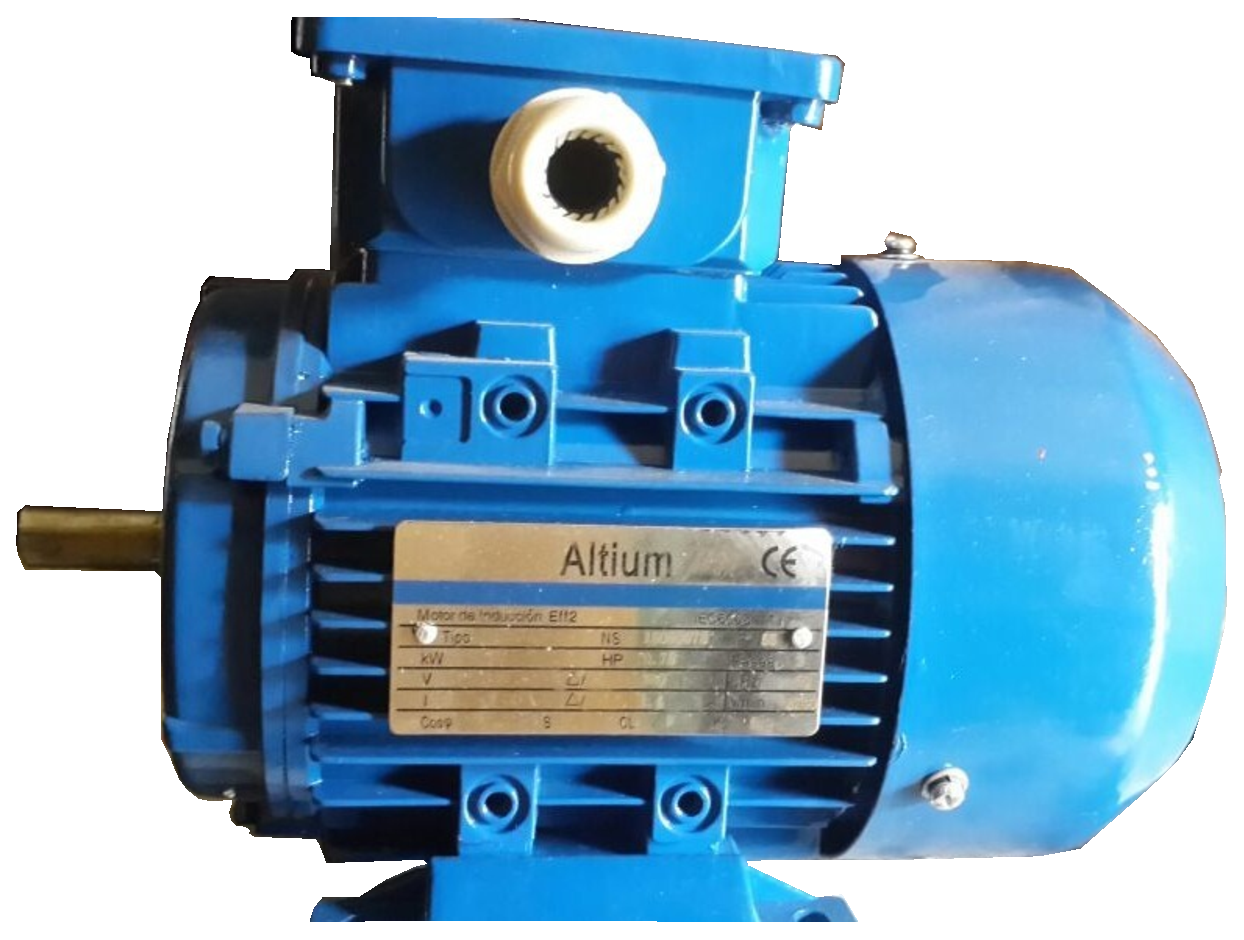
\includegraphics[scale=0.4]{motor.eps}
		\caption{Motor Altium}
		\label{fig:motor}
	\end{figure}
	\newpage

\subsection{Variador de velocidad}
Un variador de velocidad (VSD, por sus siglas en inglés Variable Speed Drive) es utilizado para controlar la velocidad de giro de un motor. \\
Para regular las revoluciones, se debe tener en cuenta las características del motor, ya que este tiene una curva propia de funcionamiento. Para seguir esta curva se emplea un variador pudiendo este ser utilizado junto con ventiladores, bombas, elevadores, portones, etc generando en estos elementos control de aceleración, frenado, seguridad, control del torque y operaciones que mejoran la eficiencia energética.

\subsubsection{Especificaciones}
El variador de velocidad que se utilizó pertenece a la marca \textbf{Schneider Electric} (Figura \ref{fig:variador}) que posee las siguientes características. \\
	\paragraph*{Altivar 312}
	\begin{itemize}
		\item 	Modelo: ATV312HU15N4
		\item   Tensión: 380-500 V
		\item 	Frecuencia: 50/60 Hz
		\item 	Potencia: 1.5kW / 2 HP
		\item 	Fases: 3
	\end{itemize}

	\begin{figure}[h!]
		\centering
		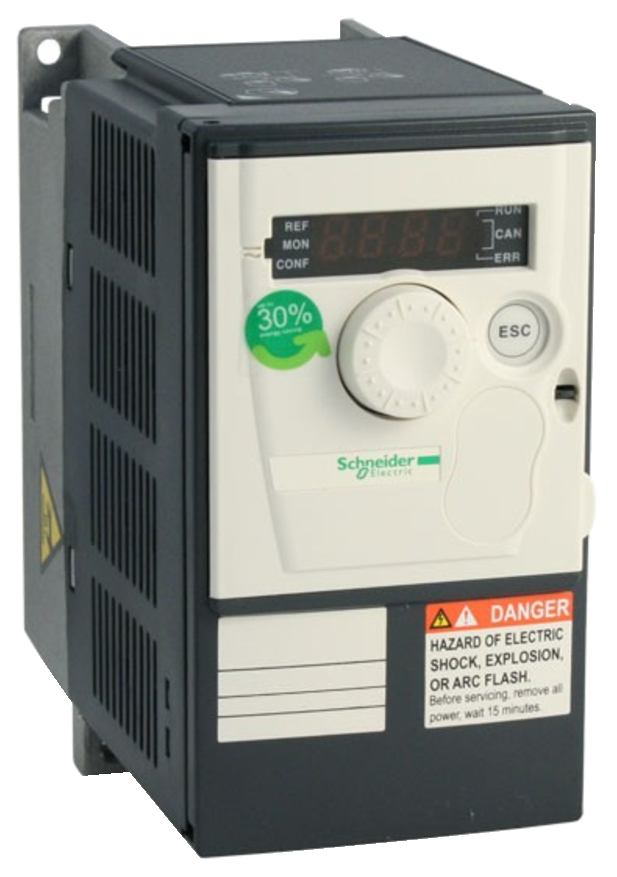
\includegraphics[scale=0.4]{variador.eps}
		\caption{Variador de velocidad Altivar 312}
		\label{fig:variador}
	\end{figure}


	\subsubsection{Configuración de parámetros primarios}
	Para realizar la configuración del motor se utilizó el software SoMove. Se descargó la ultima versión desde la página oficial de Schneider\footnote{\url{https://www.se.com/ar/es/product-range-presentation/2714-somove/}} y luego, la librería DTM correspondiente al variador a utilizar\footnote{\url{https://www.se.com/ar/es/download/document/Altivar_DTM_Library/}}. 
	\\
	Una vez realizado esto se procedió a generar un nuevo proyecto eligiendo las opciones correctas del variador.
	
	\subsubsection{Configuración de comunicación CANopen}

	\paragraph{Registros a utilizar}
	ir a ANEXO y poner la lista completa de direcciones

	\newpage



\subsection{PLC}

\subsubsection{Módulos PLC M340}



\subsubsection{Comunicación}
poner el diagrama
%El   variador   también   se   puede   controlar   en   modo   remoto.   Es   adecuado   paraaplicaciones en   los   que   los   cambios   de   variables   del   variadorse   realizan frecuentemente  durante  el proceso.  Dichos  cambios  pueden  realizarse  por  parte  del propio  operario  (mediante  potenciómetros,  interruptores,  selectores  rotativos  o  BCD, etc.).  Sin  embargo,  la  situación  más  común  es  que  los  parámetros  del  variador  los establezca  el  equipo  de  control  y  supervisión  del  proceso,  al  que  está  conectado  el variadorde  frecuencia: reguladores  de  tensión  y/o  corriente,  finales  de  carrera, pantallas de operador, etc., o incluso un ordenador personal y/o PLC. Para  el  casode  estos  controles  remotos,  la  comunicación  se  puede  realizarde  dos modos:\\Mediante un  número  determinado  de  conductores,  que  depende  de  los elementos que se tengan conectados al variador de frecuencia, por el que se transmiten señales digitales (finalesde carrera, interruptores, salidas digitales de un PLC), o analógicas (potenciómetro, salida analógica de un PLC):\\Mediante un bus de comunicaciones industriales (de 2 o 4 hilos), sobre el que se transmiten   mensajes   de   ajuste   de   parámetros   siguiendo   un   protocolo preestablecido (Modbus, CanBus, ProfiBus, EtherCat, etc.).Con 2  conductores la  comunicación  se  hace  más  lenta(modo  semidúplex),  pero  lógicamente representa un menor coste.
	
	
	

\subsection{CANopen}
\subsection{Modbus}

\subsection {HMI}
Se realizó una interfaz humana maquina con los siguientes elementos:
	\begin{itemize}
		\item boton de start(acá o en el tablero???)
		\item varias velocidades configuradas previamente
		\item inversión y señalización del mismo
		\item torque???
	\end{itemize}
	\begin{figure}[htb]
		\centering
		\includegraphics{HMIej.png}
		%\caption{Placa BME280}
		%\label{fig:BME280}
	\end{figure}

	\newpage
El   variador   también   se   puede   controlar   en   modo   remoto.   Es   adecuado   paraaplicaciones en   los   que   los   cambios   de   variables   del   variadorse   realizan frecuentemente  durante  el proceso.  Dichos  cambios  pueden  realizarse  por  parte  del propio  operario  (mediante  potenciómetros,  interruptores,  selectores  rotativos  o  BCD, etc.).  Sin  embargo,  la  situación  más  común  es  que  los  parámetros  del  variador  los establezca  el  equipo  de  control  y  supervisión  del  proceso,  al  que  está  conectado  el variadorde  frecuencia: reguladores  de  tensión  y/o  corriente,  finales  de  carrera, pantallas de operador, etc., o incluso un ordenador personal y/o PLC. Para  el  casode  estos  controles  remotos,  la  comunicación  se  puede  realizarde  dos modos:\\Mediante un  número  determinado  de  conductores,  que  depende  de  los elementos que se tengan conectados al variador de frecuencia, por el que se transmiten señales digitales (finalesde carrera, interruptores, salidas digitales de un PLC), o analógicas (potenciómetro, salida analógica de un PLC):\\Mediante un bus de comunicaciones industriales (de 2 o 4 hilos), sobre el que se transmiten   mensajes   de   ajuste   de   parámetros   siguiendo   un   protocolo preestablecido (Modbus, CanBus, ProfiBus, EtherCat, etc.).Con 2  conductores la  comunicación  se  hace  más  lenta(modo  semidúplex),  pero  lógicamente representa un menor coste.
	
	\begin{figure}[htb]
		\centering
		\includegraphics[scale=0.7]{comu.png}
		%\caption{Placa BME280}
		%\label{fig:BME280}
	\end{figure}	
	

	\paragraph{Configuración CANopen}
	imagenes. y paso a paso\\
	\\
	Modbus es un protocolo de comunicaciones situado en el nivel 7 del Modelo OSI, basado en la arquitectura maestro/esclavo o cliente/servidor, diseñado en 1979 por Modicon para su gama de controladores lógicos programables (PLCs). Convertido en un protocolo de comunicaciones estándar en la industria, es el que goza de mayor disponibilidad para la conexión de dispositivos electrónicos industriales.
%http://microelecblog.blogspot.com/2013/12/configuracion-atv312-para-red-modbus.html
	\paragraph{Configuración Modbus}
	imagenes. y paso a paso

	\subsubsection{Programación Unity Pro}
	\paragraph{Guia}
	\paragraph{Programa básico}
	\newpage

	%EL ERROR QUE TENIA CRISTIAN con ifix SE ARREGLO CON ESTO
%\url{http://www.cimexcorp.com/hasp_fix.htm}

\section{Pruebas}

\subsection{Programación variador de velocidad}


Para realizar la configuración del variador de velocidad con los parámetros del motor se utilizó el software \textit{SoMove} a través del protocolo \textit{ModBus}. Se descargó la ultima versión desde la página oficial de \textit{Schneider Electric}\footnote{\url{https://www.se.com/ar/es/product-range-presentation/2714-somove/}} y luego, la librería DTM correspondiente al variador a utilizado \footnote{\url{https://www.se.com/ar/es/download/document/Altivar_DTM_Library/}}.

Una vez instalado se procedió a generar un nuevo proyecto donde se eligió las características del variador (Figura \ref{fig:so1} y \ref{fig:so2}). El próximo paso fue realizar por medio del software la carga de los parámetros del motor (Figura \ref{fig:paramsomove}), establecer el modo de funcionamiento de las entradas y configurar el protocolo de comunicación.
\begin{figure}[h]
	\centering
	\includegraphics[width=0.9\linewidth]{somove1.png}
	\captionof{figure}{Elección de Altivar 312}
	\label{fig:so1}
\end{figure}
\begin{figure}[H]
	\centering
	\includegraphics[width=0.9\linewidth]{somove2.png}
	\captionof{figure}{Parámetros del variador}
	\label{fig:so2}
\end{figure}

\begin{figure}[H]
	\centering
	\includegraphics[width=0.7\linewidth]{images/paramsomove}
	\captionof{figure}{Lista de parámetros modificados}
	\label{fig:paramsomove}
\end{figure}


Para realizar esta primera configuración se comunicó la computadora con el variador a través del protocolo \textit{Modbus RTU} (Figura \ref{fig:pcvar}) por medio de un cable RJ45 / par trenzado y un conversor RS485 / USB (Figura \ref{fig:paramsomove1}). 
\begin{figure}[H]
	\centering
	\includegraphics[width=0.7\linewidth]{pc_var.png}
	\captionof{figure}{Diagrama de comunicación PC- variador}
	\label{fig:pcvar}
\end{figure}

\begin{figure}[H]
	\centering
	\includegraphics[width=0.9\linewidth]{paramsomove1.png}
	\captionof{figure}{Cable de comunicación}
	\label{fig:paramsomove1}
\end{figure}


\subsection{Comunicación variador de velocidad - PLC}
Para poder realizar la comunicación entre el variador y el PLC fue necesario contar con un cable RJ45 (variador) a DB9 (PLC) a través del protocolo CANopen (Figura \ref{fig:cable}), y se colocó en los finales de línea una resistencia de 120 $\Omega$ para evitar ruidos eléctricos y fenómenos de reflexión en la línea.


\begin{figure}[htbp]
    \centering
    \subfigure[Ficha entrada/salida variador]{\includegraphics[width=60mm]{canconectores.png}}
    \subfigure[Ficha entrada/salida PLC]{\includegraphics[width=80mm]{candb9.png}}
    \caption{Conexión fichas RJ45- DB9} \label{fig:cable}
    \end{figure}



\subsection{Programación Unity Pro}


Para generar la base del proyecto de trabajo, se descargó e instaló el software \textit{Unity Pro XL} y la librería DTM utilizada en el software \textit{soMove} correspondiente al variador que se posee. Una vez que fue instalado se creó y configuró un nuevo proyecto a través de los siguientes pasos.
\begin{enumerate}
	\item Se seleccionó el bastidor (Figura \ref{fig:uni0}).
	\item En la configuración gráfica del bastidor 
se introdujo los módulos
	deseados (Figura \ref{fig:uni1}) correspondientes al PLC didáctico del laboratorio (Sección \ref{sec:didac}). 
	\item Se configuró el módulo Ethernet, desde el explorador de
	proyectos se desplegó la
	carpeta \textit{Comunicación} y se creó una nueva red, Ethernet (Figura \ref{fig:inter}).
	\item Se añadió en el bus CANopen el variador utilizado (Figura \ref{fig:vcan}). En nuestro caso se eligió el ATV31 para usar los bloques de funciones de control de movimiento preestablecidos por el software.
	\item Se creó una nueva sección de lenguaje FDB para visualizar los parámetros básicos.
	\begin{itemize}
		\item Los \textit{Diagramas de Bloques de Función} consisten en un editor gráfico orientado al dibujo
		de bloques. Este se basa en la utilización de funciones reusables elementales y
		derivados.
	\end{itemize}
%\item Para realizar la conexión del PLC con la computadora se utiliza protocolo TCP/IP a través de la dirección 192.168.10.187 (Dirección que el PLC tiene configurada internamente)(Figura \ref{fig:direcc}) y (Figura \ref{fig:inter})
\end{enumerate}
	
	\begin{comment}
	que posee los siguientes módulos:
\begin{itemize}
\item BMX XBP 0400: bastidor para 4 módulos más la fuente de alimentación.
\item BMX P34 2030: CPU 340-20 Ethernet CANopen.   (Comunicación)
\item BMX ART 0414: 4 entradas TC/RTD con separación de potencial.
\item BMX DDM 16022: 8 entradas digitales, y 8 salidas digitales por transistor PNP, todas ellas aisladas.
\item BMX CPS 2000: Fuente de alimentación de 220V
\end{itemize}

	\end{comment}


\begin{center}
	\includegraphics[width=0.8\linewidth]{unit1.png}
	\captionof{figure}{Elección del bastidor}
	\label{fig:uni1}
	\includegraphics[width=0.8\linewidth]{unity1.png}
	\captionof{figure}{Módulos PLC}
	\label{fig:uni0}
\end{center}

%\begin{figure}[h]
%	\centering
%	\includegraphics[scale=1]{1.direcc.png}
%	\captionof{figure}{Dirección IP}
%	\label{fig:direcc}
%\end{figure}


\begin{figure}[h]
	\centering
	\includegraphics[width=0.9\linewidth]{2.ethern.png}
	\captionof{figure}{Dirección módulo Ethernet}
	\label{fig:inter}
\end{figure}

\begin{figure}[h]
	\centering
	\includegraphics[scale=0.8]{vcan.png}
	\captionof{figure}{Configuración variador CANopen}
	\label{fig:vcan}
\end{figure}


Una vez que se completó la configuración de la comunicación variador - PLC se procedió a crear un HMI simple en\textit{ iFix} (Figura \ref{fig:previo}), el cual fue utilizado para interactuar y observar diversos parámetros, modificar velocidades, observar señales luminosas y ver distintos valores proporcionados por el variador de velocidad.
 
\begin{figure}[H]
	\centering
	\includegraphics[width=0.9\linewidth]{3.previo.png}
	\captionof{figure}{HMI simple}
	\label{fig:previo}
\end{figure}

Para observar en el HMI se utilizó los MFB del software \textit{UnityPro} (Figura \ref{fig:read}), los cuales necesitan de un bloque maestro ``CAN\_HANDLER'' el cual permite comprobar la comunicación \textit{CANopen}.

Otros de los bloques más utilizados dentro del programa fue ``MC\_READPARAMETER'' que se utiliza para leer, mediante mensajes SDO, una variable del variador definida en una dirección \textit{CANopen} dada por el fabricante \cite{ComManual}.

\begin{figure}[H]
	\centering
	\includegraphics[width=0.9\linewidth]{4.read.png}
	\captionof{figure}{Programa con bloques MFB}
	\label{fig:read}
\end{figure}



\subsubsection{Entradas analógicas}
En el rack del PLC se encuentra un módulo AMI0410 el cual consiste en cuatro entradas analógicas (Tensión/Corriente) aisladas del siguiente tipo:
\begin{itemize}
	\item Corriente +/- 20 mA
\item 	Corriente 0 a 20 mA
\item 	Corriente 4 a 20 mA
\item 	Tensión +/- 10 V
\item 	Tensión +/- 5 V
\item 	Tensión 0 a 10 V
\item 	Tensión 0 a 5 V
\item 	Tensión 1 a 5 V
	
\end{itemize}

El módulo dispone de 20 bornes accesibles al usuario dónde el diagrama de conexión tanto para entradas de tensión o de corriente es el mostrado en la figura \ref{fig:modulo}.

Para realizar la configuración en \textit{Unity PRO} se elige, de las opciones nombradas anteriormente, la que se utilizó en este caso de 4 a 20 mA y el escalado predefinido de fábrica de 0 a 10000 cuentas, pero modificable por el usuario entre -32768 a 32767 ya que la resolución de las entradas analógicas es de 16 bits. También se agregó un filtro de primer orden a cada entrada por software (Figura \ref{fig:param}).

Con el rango de cuentas del módulo determinado, se requirió escalar la variable para obtener el valor físico y así utilizarla para la visualización y control del banco de pruebas.

Para el escalado de la señal de entrada se realizó un nuevo bloque FB derivado, a partir elementos primarios, para evitar realizar un proceso repetitivo en el escalado de varias señales (Figura \ref{fig:escalado}).

En la variable de entrada se coloca la señal que se desea escalar, en los límites de entrada se escribe el rango del módulo visto anteriormente, y en los límites de salida, los escalados obtenidos del instrumento que se utilizó.

 Finalmente, a la salida del bloque se obtuvo el valor físico visualizado o transmitido por el instrumento.

\begin{figure}[H]
	\centering
	\includegraphics[width=0.6\linewidth]{modulo.png}
	\captionof{figure}{Módulo AMI0410}
	\label{fig:modulo}
\end{figure}
\begin{figure}[H]
	\centering
	\includegraphics[width=0.9\linewidth]{param.png}
	\captionof{figure}{Rango y escalado}
	\label{fig:param}
\end{figure}

\begin{figure}[H]
	\centering
	\includegraphics[width=0.9\linewidth]{escalado.png}
	\captionof{figure}{Bloques de escalado}
	\label{fig:escalado}
\end{figure}


\subsubsection{Entradas analógicas para termocuplas o RTD}
Se utilizó el módulo ART0414 que consiste en cuatro entradas aisladas en las que se pueden conectar sensores de temperatura del tipo termocupla y RTD con las siguientes características:
\begin{itemize}
	\item RTD IEC Pt100/Pt1000, US/JIS Pt100/Pt1000, Cu10, Cu50, Cu100, Ni100/Ni1000 en 2, 3 o 4 conductores
	\item Termoelemento del tipo B, E, J, K, L, N, R, S, T, U
\item 	Tensión $+/-$ 40 mV a 1,28 V
	
\end{itemize}

Para la conexión de estos sensores se utiliza el accesorio TELEFAST ABE-7CPA412 (Figura \ref{fig:ABE}) y se tiene las formas de conexión, de la figura \ref{fig:ABE2}, dependientes del tipo de sensor.

\begin{figure}[H]
	\centering
	\includegraphics[width=0.9\linewidth]{ABE.png}
	\captionof{figure}{Accesorio TELEFAST ABE-7CPA412}
	\label{fig:ABE}
\end{figure}
\begin{figure}[H]
	\centering
	\includegraphics[width=0.9\linewidth]{ABE2.png}
	\captionof{figure}{Conexión según sensor}
	\label{fig:ABE2}
\end{figure}

Para configurar en \textit{Unity Pro} se seleccionó en \textit{rango} las características del sensor y en \textit{escala} se modificó los valores para que coincidan con los máximos y mínimos del sensor. En el caso de RTD y termocupla los valores son múltiplos de 10 respecto a la temperatura en °C o °F. 

En la imagen \ref{fig:ABE3} se observa dos elementos ya que se probó realizar la configuración con una termocupla y un RTD. Finalmente se eligió el RTD PT1000 dónde el valor obtenido se divide por 10 y se genera el valor de temperatura en °C con un decimal  (Figura \ref{fig:ABE3}).

\begin{figure}[H]
	\centering
	\includegraphics[width=0.9\linewidth]{ABE3.png}
	\captionof{figure}{Rango y escalado}
	\label{fig:ABE3}
\end{figure}

\begin{figure}[H]
	\centering
	\includegraphics[width=0.6\linewidth]{ABE4.png}
	\captionof{figure}{Bloque de escalado}
	\label{fig:ABE4}
\end{figure}

\subsubsection{Medición de caudal}
Según la cantidad de flujo que pase por el caudalímetro, este entregaría pulsos que debían ser leídos con un módulo externo del PLC por la baja resolución que posee. Para esto se planteó utilizar un ESP8266 como interfaz para obtener los pulsos, colocarlos en un registro y enviarlos por un servidor Modbus TCP cada 20ms al PLC. En la sección de programación del PLC se realizó las cuentas correspondientes para realizar la conversión de pulsos a caudal (Figura \ref{fig:modtcp}). Tanto para el módulo, como para el caudalímetro se usó una fuente externa de 3,3 V de alimentación.
\begin{figure}[htbp]
	\centering
	\includegraphics[scale=1]{esp_mod.png}
	\captionof{figure}{Diagrama de flujo del caudalimetro} 
	\label{fig:modtcp}
\end{figure}
\newpage

%\url{
%https://download.schneider-electric.com/files?p_enDocType=User+guide&p_File_Name=35010608_K01_000_11.pdf&p_Doc_Ref=35010608K01000}


\section{HMI SCADA}
\begin{tcolorbox}[colback=blue!5!white,colframe=blue!75!black,title=HMI - SCADA]
	Ambas tecnologías, HMI y SCADA, son utilizadas en conjunto en la industria de la automatización. SCADA proporciona funciones de supervisión, alarmas y control, mientras que HMI proporciona las herramientas que necesita para desarrollar imágenes que los operadores pueden usar para monitorear su proceso. El HMI se utiliza para monitorear o visualizar lo ejecutado por SCADA.
\end{tcolorbox}

\subsection{MBE}
\subsection{iFix}
\subsubsection{Guia}
\subsubsection{Programa}


Se realizó una interfaz humana maquina con los siguientes elementos:
\begin{itemize}
	\item boton de start(acá o en el tablero???)
	\item varias velocidades configuradas previamente
	\item inversión y señalización del mismo
	\item torque???
	\item HMI
	      \subitem Alarmas
	      \subitem Información en tiempo real
	      \subitem Histórico de datos
	      \subitem Control general del banco
\end{itemize}
\begin{figure}[htb]
	\centering
	\includegraphics{HMIej.png}
	%\caption{Placa BME280}
	%\label{fig:BME280}
\end{figure}

\subsubsection{Alarmas- iHistorian}

\section{Banco de pruebas}
Como se nombró en el objetivo, se busca realizar el control de caudal o presión de un sistema hidráulico. Para esto fue necesario realizar la implementación de un banco de pruebas que cuente de tres partes (Figura \ref{fig:bancofull}).
\begin{itemize}
	\item Soporte para el motor y variador de velocidad,  diseñado y construido por el profesor Gerardo Arthz. A estos elementos se realizó las correspondientes conexiones, y se agregó elementos adicionales: 3 señales luminosas, llave selectora de dos puntos para seleccionar el modo de comunicación, llave selectora de tres puntos (encendido y sentido del motor) y un pulsador de parada de emergencia (Figura \ref{fig:banco}(a)).
	Tanto el motor y los elementos adicionales fueron cableados (Figura \ref{fig:banco}(b)) hacia las borneras del variador de velocidad y se tuvo en cuenta para esto las características y funciones del bornero de control proporcionado por el manual del variador de velocidad\cite{InstaManual}. 
	
	\item Soporte para una bomba en desuso, de características no conocidas con su bobinado quemado.
	\item Circuito hidráulico, que incluye un tanque, válvulas y sensores de caudal y presión.
\end{itemize}




\begin{figure}[htb]
	\centering
	\includegraphics[width=0.9\linewidth]{bancofull.png}
	\captionof{figure}{Banco de pruebas completo}
	\label{fig:bancofull}
\end{figure}


\begin{figure}[H]
	\centering
	\subfigure[]{\includegraphics[angle=-90,width=70mm]{banc1 (1)}}
	\subfigure[]{\includegraphics[angle=-90,width=70mm]{images/banc1 (2)}}
	\caption{Banco de Pruebas} \label{fig:banco}
\end{figure}

\subsubsection{Transmisor de presión}
Para este proyecto se utilizan dos transmisores de presión de montaje en línea modelo EJA530E de la familia  DPharp de Yokogawa (Figura \ref{fig:transd}.a).\\
Las características del EJA530E son:
\begin{itemize}
	\item Precisión: ±0,055\% de precisión
	\item Fiabilidad: ±0,1\% Estabilidad por 10 años
	\item Tiempo de respuesta: 90mseg.
	\item Lazo de corriente de 4-20mA
	\item Se puede configurar en la unidad necesaria, en este caso mBar.
\end{itemize}


\subsubsection{Sensor de caudal}
Se utilizó un sensor de caudal (Figura \ref{fig:transd}.b) genérico con las siguientes características:
\begin{itemize}
	\item Rango de caudal: 2- 60L/min
	\item Máxima presión de agua: 1,75MPa
	\item Conversión de caudal: aprox 477pulsos/L $\pm$ 10\%
\end{itemize}


\begin{figure}[htbp]
	\centering
	\subfigure[Transmisor de presión]{\includegraphics[height=40mm]{tran_pre.png}}
	\subfigure[Sensor de caudal]{\includegraphics[height=40mm]{sens_pre.png}}
	\caption{Transmisores} \label{fig:transd}
\end{figure}





\subsection{Diagrama}
Colocar el diagrama \fcolorbox{red}{yellow}{tipo imagen} pero ver si se agrega el variador y el plc FIGURA\ref{fig:diag}

\begin{figure}[htb]
	\centering
	\includegraphics[width=0.9\linewidth]{diag.png}
	\captionof{figure}{Diagrama p\&id}
	\label{fig:diag}
\end{figure}

\subsection{Presupuesto}
\fcolorbox{red}{yellow}{falta lo de la bomba}
\url{https://docs.google.com/spreadsheets/d/1mFoNvgJXUdL2bNnspaBJ_wS5fFA1y1c8fTO9Rfod7H0/edit#gid=0}

\newpage

\section{Conclusiones}

\clearpage
\newpage

\section{Mejoras futuras}
En un futuro se espera que alumnos de la carrera realicen mejoras en el banco de pruebas, por ejemplo:
\begin{itemize}
	\item Mejorar la distancia entre los sensores y los accesorios del sistemas, como válvulas o codos para que el fluido no se torne turbulento.
	\item Implementar sistemas sonoros o visuales de las alarmas.
	\item Generar una página web para observar los datos en tiempo real y/o manejar de forma remota.
	\item Realizar otro anexo no hidráulico para colocar al motor- variador y generar un nuevo banco de pruebas.
	\item Generar nuevas formas de perturbación a los sistemas.
	\item Implementar un sistema para controlar presión o caudal por medio de válvulas proporcionales.
	\item Realizar perturbaciones controladas y repetibles con válvulas proporcionales.
	\item Reemplazar bomba por una en mejor estado.
	\item Realizar pruebas de caudal y presión a mayor frecuencia.
\end{itemize}

\newpage
\section{Conclusiones}
Se concluye que el banco de pruebas construido es una herramienta útil para alumnos de las carreras de ingeniería que sigan ramas orientadas al control automatizado, ya que se tiene la posibilidad de generar perturbaciones en el sistema y observar distintas respuestas.

Se generó un sistema SCADA dónde se puede observar diversas variables en tiempo real y realizar estudios de ellas a través de datos históricos. Además, en la pantalla, se puede observar distintos tipos de anomalías causadas por el variador y los instrumentos utilizados en el proyecto, para facilitar la detección de errores y poder solucionarlos adecuadamente.

Se logró tener control eficaz sobre tres variables distintas mediante la variación de la frecuencia del motor, dónde esta es la única acción de control en el banco de pruebas.

Finalmente, la realización del proyecto tuvo un gran aporte para consolidar los conocimientos obtenidos durante la cursada de la materia \textit{Automatización Industrial} y también para el crecimiento personal y profesional.



\newpage

\section{Bibliografía}

\section{Anexos}
\newpage
\section{Anexo: Diagrama P \& ID} \label{anexopid}
	
	
\begin{figure}[h!]
	\centering
	\includegraphics[scale=0.9 ,angle =90]{diag.png}
	\captionof{figure}{Diagrama p\&id}
\end{figure}

\newpage
\section{Anexo: Tabla de Direcciones ModBus} \label{Anexo1}


\begin{longtable}{|p{1.2cm} |p{4cm} |p{4cm} |p{1.5cm} |p{3.2cm} |}
	\caption{Tabla de variables y direcciones}
	\label{tab:direc}  \\
	
	\hline
	\multicolumn{1}{|c|}{\textbf{\begin{tabular}[c]{@{}c@{}}Tipo de \\ variable\end{tabular}}} & \multicolumn{1}{c|}{\textbf{TAG}} & \multicolumn{1}{c|}{\textbf{Descripción}} & \multicolumn{1}{c|}{\textbf{\begin{tabular}[c]{@{}c@{}}Tipo de \\ dato\end{tabular}}} & \multicolumn{1}{c|}{\textbf{Dirección}} \\ \hline
	\endfirsthead
	
	\multicolumn{5}{c}%
	{{\bfseries \tablename\ \thetable{} -- continuación}} \\
	\hline
	\multicolumn{1}{|c|}{\textbf{\begin{tabular}[c]{@{}c@{}}Tipo de \\ variable\end{tabular}}} & \multicolumn{1}{c|}{\textbf{TAG}} & \multicolumn{1}{c|}{\textbf{Descripción}} & \multicolumn{1}{c|}{\textbf{\begin{tabular}[c]{@{}c@{}}Tipo de \\ dato\end{tabular}}} & \multicolumn{1}{c|}{\textbf{Dirección}} \\ \hline
	\endhead
	
	\hline \multicolumn{5}{|r|}{{Sigue en la página siguiente}} \\ \hline
	\endfoot
	
	%\hline \hline
	\endlastfoot
	

	DO & PID\_XSMA0 & Habilitar control automatico manual & Boolean & Device0:000003 \\ \hline
	DO & VSD\_XSM0 & Marcha desde el hdmi & Boolean & Device0:000004 \\ \hline
	DO & VSD\_XST0 & Parada desde SCADA & Boolean & Device0:000005 \\ \hline
	DO & PLC\_XSDES & Desenclave de bomba & Boolean & Device0:000006 \\ \hline
	DO & PID\_XSA0 & PID modo automatico & Boolean & Device0:000008 \\ \hline
	DO & PID\_XSM0 & PID modo manual & Boolean & Device0:000009 \\ \hline
	DO & VSD\_XSFO & Restablecer fallas VSD & Boolean & Device0:000010 \\ \hline
	DI & VSD\_YHS0 & Parada de emergencia fisico & Boolean & Device0:000011 \\ \hline
	DI & VSD\_YLR0 & Modo fisico o scada & Boolean & Device0:000012 \\ \hline
	DI & PID\_YMA0 & Estado manual automatico & Boolean & Device0:000013 \\ \hline
	DI & PID0PIT1\_XRST & Restablecer valores PID & Boolean & Device0:000014 \\ \hline
	DI & PID0PIT2\_XRST & Restablecer valores PID & Boolean & Device0:000015 \\ \hline
	DI & PID0FT1\_XRST & Restablecer valores PID& Boolean & Device0:000016 \\ \hline
	AI & FT01 & Caudal & Float & Device0:400001 \\ \hline
	AI & VSD\_AI1C & Valor del pote & Float & Device0:400003 \\ \hline
	AI & VSD\_IC000 & Corriente & Float & Device0:400005 \\ \hline
	AI & VSD\_SC000 & Frecuencia & Float & Device0:400007 \\ \hline
	AI & VSD\_JC000 & Potencia & UInt & Device0:400009 \\ \hline
	AI & VSD\_WC000 & Torque & UInt & Device0:400011 \\ \hline
	AI & VSD\_EC000 & Voltaje & Float & Device0:400013 \\ \hline
	AI & PIT02 & Presion2 & Float & Device0:400015 \\ \hline
	AI & PIT01 & Presion1 & Float & Device0:400017 \\ \hline
	AI & VSD\_SC001 & Velocidad & UInt & Device0:400019 \\ \hline
	AI & TE001 & Temperatura & Float & Device0:400021 \\ \hline
	AI & PID\_SY000 & Accion de control & Float & Device0:400023 \\ \hline
	AI & VSD\_R\_ERR & Errores, tabla de errores & UInt & Device0:400025 \\ \hline
	AI & PID0PIT1\_TD\_LAG & P1 TD LAG & Float & Device0:400047 \\ \hline
	AI & PID0PIT2\_TD\_LAG & P2 TD LAG & Float & Device0:400049 \\ \hline
	AI & PID0FT1\_TD\_LAG & F1 TD LAG & Float & Device0:400051 \\ \hline
	AI & PID\_SR00 & Valor manual, control desac & Float & Device0:400053 \\ \hline
	AI & PID0PIT1\_SP & Valor Ref P1 & Float & Device0:400057 \\ \hline
	AI & PID0PIT2\_SP & Valor Ref P2 & Float & Device0:400059 \\ \hline
	AI & PID0FT1\_SP & Valor Ref F1 & Float & Device0:400061 \\ \hline
	AI & PID0PIT1\_KI & P1 KI & Float & Device0:400063 \\ \hline
	AI & PID0PIT1\_KP & P1 KP & Float & Device0:400065 \\ \hline
	AI & PID0PIT1\_KD & P1 KD & Float & Device0:400067 \\ \hline
	AI & PID0PIT2\_KI & P2 KI & Float & Device0:400071 \\ \hline
	AI & PID0PIT2\_KP & P2 KP & Float & Device0:400073 \\ \hline
	AI & PID0PIT2\_KD & P2 KD & Float & Device0:400075 \\ \hline
	AI & PID0FT1\_KI & F1 KI & Float & Device0:400077 \\ \hline
	AI & PID0FT1\_KP & F1 KP & Float & Device0:400079 \\ \hline
	AI & PID0FT1\_KD & F1 KD & Float & Device0:400081 \\ \hline
	AI & PID\_SEL & Seleccionar control P1 P2 F1 & UInt & Device0:400083 \\ \hline
	DR & VSD\_ETI & Motor encendido o apagado & Boolean & Device0:400101:4 \\ \hline
	DR & YS\_AP & Alta presion & Boolean & Device0:400103:0 \\ \hline
	DR & YS\_SC & Sin Caudal & Boolean & Device0:400103:1 \\ \hline
	DR & YS\_SP1 & Sin Sensor P1 & Boolean & Device0:400103:2 \\ \hline
	DR & YS\_SP2 & Sin Sensor P2 & Boolean & Device0:400103:3 \\ \hline
	DR & YS\_AT & Alta Temp & Boolean & Device0:400103:4 \\ \hline
	DR & FT01\_YCOM & Sin Caudal & Boolean & Device0:400103:5 \\ \hline
	DR & VSD\_YCOM & Sin comu con variador & Boolean & Device0:400103:6 \\ \hline
	%	\\*
	%	\caption{Tabla de variables y direcciones}
	%	\label{tab:direc}  	
	
	
\end{longtable}

\newpage

\section{Anexo: Manual BANCO-SCADA}
\subsection{Características generales}
\begin{itemize}
	\item Utilizado en sistema operativo Windows 10 o mayor.
	\item Posibilidad de utilizar el banco de pruebas de modo remoto o local.
	\item Generado para controlar tres variables distintas, dos de presión o caudal.
\item Posibilidad de generar perturbaciones en el sistema para observar distintas respuestas.
	\item Fácil de transportar.
\item Posibilidad de guardar valores como históricos y ver datos en tiempo real.
\end{itemize}


\subsection{Guía de uso}
\begin{enumerate}
	\item Conectar el banco de pruebas con los respectivos sensores y transductores en el módulo correspondiente del PLC.
	\item Conectar cable Ethernet en el PLC a un router o PC.
	\item Alimentar el sistema con alimentación trifásica y 220V.
	\item Abrir iFix y la tabla de variables y el archivo con extensión .mbe dónde se procederá a conectar el sistema SCADA a la misma red en la que se encuentra el PLC.
	\item Comprobar comunicación al correr SCADA.
\end{enumerate}

\subsubsection{Pantalla PRINCIPAL}

\begin{figure}[h!]
	\centering
	\includegraphics[width=0.9\linewidth]{pantalla1.png}
	\captionof{figure}{Pantalla principal}
	\label{fig:pantalla1}
\end{figure}
\begin{figure}[h!]
	\centering
	\includegraphics[width=0.6\linewidth]{p_partes.png}
	\captionof{figure}{Partes del sistema SCADA}
	\label{fig:partes}
\end{figure}

\paragraph{Diagrama del banco de pruebas}
Se observan los valores de presión y caudal en un diagrama similar al banco de prueba físico. A la izquierda se mostrará el último error el cúal puede observarse en la tabla que se abre al hacer click en el botón A. Si se desea restaurar el valor se debe presionar el botón B (Figura \ref{fig:pp1}).
\begin{figure}[h!]
	\centering
	\includegraphics[width=0.6\linewidth]{p_p1.png}
	\captionof{figure}{Subpantalla 1}
	\label{fig:pp1}
\end{figure}

\paragraph{Estado del variador - Motor}
En esta sección se ve de forma lumínica en color rojo si el motor está prendido indica señal de cuidado o alerta; mientras que en color verde que el motor está apagado. Se observan variables de velocidad del motor, frecuencia del motor, temperatura obtenida por el termistor, corriente, torque y potencia consumida por el motor.
\paragraph{Alarmas}
Sección destinada al alarmero dónde muestra el período de tiempo que ocurrió el hecho, el nombre de la variable y el valor alcanzado.
\paragraph{Modo remoto/ Modo local}
\begin{itemize}
	\item Modo Local\\
	Si la llave selectora del banco de pruebas se encuentra seleccionado el modo local, se observará el cartel en esta sección centrado que expresará que se encuentra en modo local (Figura \ref{fig:localremoto}.a).
	\item Modo Remoto\\
	Si la llave selectora del banco de pruebas se encuentra seleccionado el modo remoto, el sistema está preparado para recibir órdenes desde el sistema SCADA. El motor puede encenderse con velocidad 0 al presionar la tecla A o encender a una velocidad preestablecida colocando previamente un valor entero en RPM entre 0 y 3600 y luego presionar la tecla A (Figura \ref{fig:localremoto}.b). 
	
	Si se desea se puede abrir cada ventana del lazo de control (Figura \ref{fig:LC}) botones B dónde muestra el valor de cada variable PID, pudiéndose colocar otros valores mientras que se use la coma como separador decimal. Con el botón C, se podrá restablecer los valores del PID cuyos valores fueron fijados al momento de realizar el proyecto, dónde las respuestas se muestran en las figuras PONER TIPO LA COMPARACION DE PID PERO CON SOLO EL QUE SE UTILIZA Y Q SE LEEAN LOS VALORES DE PID. 
	
	Al presionar el botón automático (D), se cierra el lazo del sistema y puede establecerse la presión o caudal deseado en E, dónde la coma será el separador decimal y los rangos serán según tabla \ref{tab:rang}. En caso de presionar y que quede manual (D) los valores se establecerán según \textit{Manual} (Figura \ref{fig:localremoto}.b). 
\end{itemize}

\begin{figure}[htbp]
	\centering
	\subfigure[Modo local]{\includegraphics[width=60mm]{p_4c.png}}
	\subfigure[Modo remoto]{\includegraphics[width=60mm]{p_4b.png}}
	\caption{Subpantalla 4} \label{fig:localremoto}
\end{figure}

\begin{figure}[h!]
	\centering
	\includegraphics[width=60mm]{p_4a.png}
	\captionof{figure}{Modo lazo cerrado}
	\label{fig:LC}
\end{figure}
\begin{table}[]
	\centering
	
	\begin{tabular}{|cc|l|c|}
		\hline
		\multicolumn{2}{|l|}{\textbf{Variable}} & \textbf{Rango} & \multicolumn{1}{l|}{\textbf{Unidades}} \\ \hline
		\multicolumn{1}{|c|}{\textbf{PIT001}} & Presión & 60 - 930 & mbar \\ \hline
		\multicolumn{1}{|c|}{\textbf{PIT002}} & Presión & 60 - 700 & mbar \\ \hline
		\multicolumn{1}{|c|}{\textbf{FT001}} & Caudal & 2 - 11,7 & l/min \\ \hline
	\end{tabular}
\caption{Rangos de las variables}
\label{tab:rang}
\end{table}

\paragraph{Fallas y ventanas de gráficos}
En la pantalla 5 se observan los carteles de eventuales fallas que puedan ocurrir en el sistema, pudiéndolo reanudar con el botón que tiene la letra R.

Otra de las cosas que tiene esta subpantalla es la fecha y hora y dos botones dónde al presionarlos se abren pantallas para observar gráficamente datos en tiempo real o de forma histórica.

\subsubsection{Pantalla datos en tiempo real}
En la figura \ref{fig:scadaTR} se puede observar la pantalla de los datos en tiempo real (la imagen no corresponde a valores reales tomados durante las pruebas).
\begin{figure}[h!]
	\centering
	\includegraphics[width=1\linewidth]{scadaTR.png}
	\captionof{figure}{Pantalla datos en tiempo real}
	\label{fig:scadaTR}
\end{figure}

\subsubsection{Pantalla datos histórico}

Para interpretar datos históricos se puede por dos métodos, uno es generar un archivo .txt y el otro es de forma gráfica. 
Se generó una pantalla SCADA prediseñada de \textit{iFix} dónde al conectar con el servidor \textit{Historian}, busca los datos históricos de la variable elegida y guarda un archivo \textit{.txt} con el horario y valores. Se puede elegir más de una variable, pero se debe tener en cuenta que no se generan columnas nuevas sino que generará en el mismo archivos más filas (Figura \ref{fig:grafhist} a).\\
Otra de las opciones es observar datos históricos en un gráfico de tiempo, estas variables están preestablecidas y son las presiones y el caudal con sus respectivos valores de referencias (Figura \ref{fig:grafhist} b).


\begin{figure}[htbp]
	\centering
	\subfigure[Gráficos de datos históricos]{\includegraphics[width=1\linewidth]{scada3.png}}
	\subfigure[Guardado de datos históricos]{\includegraphics[width=1\linewidth]{scada33.png}}
	\caption{Datos históricos} \label{fig:grafhist}
\end{figure}





\newpage

\end{document}